\documentclass[
	parskip=half,
	a4paper,
]{scrarticle}

\usepackage{xcolor}
\definecolor{seeblau}{HTML}{00A9E0}
\definecolor{seegrau}{HTML}{9AA0A7}

\definecolor{seeblau1}{HTML}{CCEEF9}
\definecolor{seeblau2}{HTML}{A6E1F4}
\definecolor{seeblau3}{HTML}{59C7EB}
\definecolor{seeblau4}{HTML}{00A9E0}
\definecolor{seeblau5}{HTML}{008ECE}


\usepackage{graphicx}
\usepackage{amsmath}
\usepackage{subcaption}
\usepackage{wrapfig}
\usepackage[english]{babel}
\usepackage{blindtext}
\usepackage{microtype}
\usepackage{siunitx}
\usepackage[utf8]{inputenc}
\usepackage{csquotes}
\usepackage{nicefrac}
\usepackage[T1]{fontenc}
\usepackage{amsfonts}
\usepackage{amssymb}
\usepackage{tikz}
\usepackage{parskip}

\usepackage{libertinus, libertinust1math}
\usepackage[sfdefault]{biolinum}
\usepackage{roboto}

\setkomafont{disposition}{\normalfont\sffamily}

% set margins
\usepackage{geometry}
\geometry{
	a4paper,
	left=2.5cm,
	right=2.5cm,
	top=2.5cm,
	bottom=2.5cm
}

% caption
\usepackage{caption}
\captionsetup{
	% font={sf},
	labelfont={sf, bf, color=seeblau},
	labelsep=quad,
	labelformat=simple,
}

% links
\usepackage{hyperref}
\hypersetup{
	colorlinks=true,
	linkcolor=seeblau,
	citecolor=seeblau,
	urlcolor=seeblau,
	% hidelinks=true
}

% bibliography
\usepackage[
	style=numeric-comp, % comp = compressed 4,5,6,7 -> 4-7
	sorting=none,		% Sort by appearance
	% autocite = superscript,
	% backref=true,
	hyperref=true,
	url=true,
	maxbibnames=100
]{biblatex}

\usepackage{float}
% \floatplacement{figure}{h}
% \floatplacement{table}{H}

% loosen float placement rules
\renewcommand{\topfraction}{0.8}
\renewcommand{\bottomfraction}{.8}
\renewcommand{\textfraction}{0.1}
\renewcommand{\floatpagefraction}{.9}
% make floats less likely to be placed on a separate page
\setcounter{totalnumber}{9}
\setcounter{topnumber}{9}
\setcounter{bottomnumber}{9}

% decrease space between floats and text
\setlength{\textfloatsep}{0.25cm}
\setlength{\floatsep}{0.25cm}

% decrease space after disposition
\RedeclareSectionCommands[
	afterskip=1px
]{section, subsection, subsubsection}

\usepackage{adjustbox}

\usepackage{datetime}
\newdateformat{dotdate}{
	\twodigit{\THEDAY}.\twodigit{\THEMONTH}.\THEYEAR
}
\newdateformat{monthyeardate}{%
  \monthname[\THEMONTH] \THEYEAR}


% header and footer
\usepackage[
  markcase=noupper
]{scrlayer-scrpage}% activates pagestyle scrheadings automatically
\clearpairofpagestyles
\setkomafont{pageheadfoot}{\normalfont\sffamily}
\setkomafont{pagenumber}{\normalfont\sffamily}
% \chead*{\color{seegrau} Draft \dotdate\today}
\ofoot*{\pagemark}
\ohead*{\rightmark}


\usepackage{ifthen}
\newcommand{\markieren}[4]{
	\ifthenelse{\equal{#1}{}}{}{\adjustbox{padding=3pt, bgcolor=seeblau1, margin=-1pt}{\strut{\sffamily\robotoMedium{#1}}}\\}
  \ifthenelse{\equal{#2}{}}{}{\adjustbox{padding=3pt, bgcolor=seeblau2, margin=-1pt}{\strut{\sffamily\robotoMedium{#2}}}\\}
	\ifthenelse{\equal{#3}{}}{}{\adjustbox{padding=3pt, bgcolor=seeblau3, margin=-1pt}{\strut{\sffamily\robotoMedium{#3}}}\\}
	\ifthenelse{\equal{#4}{}}{}{\adjustbox{padding=3pt, bgcolor=seeblau4, margin=-1pt}{\strut{\sffamily\robotoMedium{#4}}}}
}

\addbibresource{../literature.bib}
\begin{document}

\title{Ultrafast Photoluminescence}
\author{Leon Oleschko}
\date{\dotdate\today}

\begin{titlepage}
    \sffamily
    \vspace*{3cm}
    {
        \fontsize{32}{32}
        \markieren{}{}{Ultrafast}{Photoluminescence}
    }
    \vspace{.25cm}\\
    {
        \Large
        Leon Oleschko\\
        supervised by Peter Baum
        \vspace{.05cm}\\
        \dotdate\today\\
        \textbf{Draft}\\
        \vspace{.05cm}\\
        \normalsize
        Projekt Praktikum\\
        Universität Konstanz
    }
    \vfill
    {
        \normalfont\normalsize
    }
    \vfill
    \begin{flushright}
        Available at \url{www.github.com/leoole100/projekt-praktikum}.
    \end{flushright}
\end{titlepage}

% {
% 	\sffamily
% 	\hypersetup{hidelinks}
% 	\tableofcontents
% }

\clearpage

\section{Introduction}


\clearpage
\section{Model}
\begin{figure}[b]
    \centering
    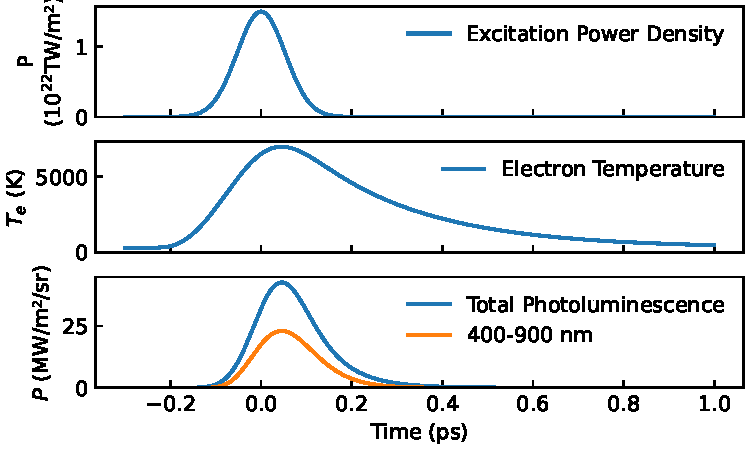
\includegraphics{../analysis/figures/model.time_evolution.pdf}
    \caption{}
    \label{fig:timeevolution}
\end{figure}

The dynamics the ultrafast Photoluminescence can be modelled using a simplified two temperature model. 
A excitation pulse with a absorbed power density $P_V(t) = P_\text{exc}(t) / V$ is absorbed by the material in a volume $V$.
This raises the electron temperature $T_e$ according to the electronic heat capacity $T_e(t)$. 
Then the electrons are cooled by coupling with a electron–phonon relaxation time $\tau$ to lattice at a constant temperature $T_l$.
This is described by the ordinary differential equation
\begin{equation}
    \frac{\mathrm d T_e(t)}{\mathrm d t}
    =
    \frac{P_V(t)}{C_e(T_e)}
    -\frac{T_e(t) - T_l}{\tau}.
    \label{eq:Te}
\end{equation}

This is solved in \autoref{fig:timeevolution} with realistic excitation values of a absorbed power density of $U_\text{abs} = \SI{2e9}{J/m^3}$ spread in a gaussian pulse with a full width half maximum (FWHM) of $t=\SI{250}{fs}$ and the electronic heat capacity \cite{nihiraTemperatureDependenceLattice2003} and the coupling time $\tau=\SI{250}{fs}$ \cite{stangeHotElectronCooling2015} of graphite.



The emitted spectral radiance $L_\lambda$ can be calculated using Plank's law
\begin{equation}
    L_\lambda(\lambda,T)
    = \epsilon(\lambda) \frac{2hc^{2}}{\lambda^{5}}
      \frac{1}{\exp\bigl(hc / \lambda k_{\mathrm B}T\bigr)-1}.
\end{equation}

The emissivity $\epsilon$ is assumed to be unity \cite{sapritskyBlackbodyRadiometry1995}.

The time evolution of the total radiance $L$ and the radiance visible by common detectors is also shown in \autoref{fig:timeevolution}.

\begin{figure}
    \centering
    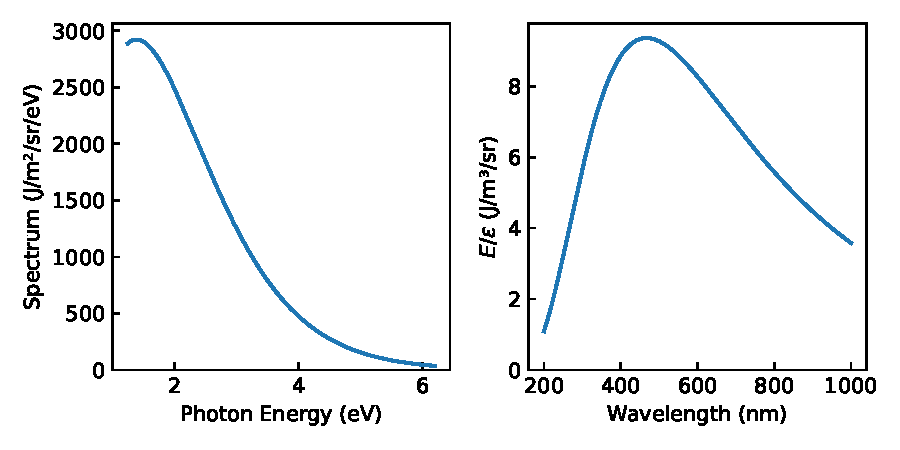
\includegraphics{../analysis/figures/model.spectrum.pdf}
    \caption{}
    \label{fig:model_spectrum}
\end{figure}

We define the spectrum $H_\lambda(\lambda)$ as the spectral radiant energy density, i.e. the spectral radiance $L_\lambda(\lambda, T)$ integrated over the pulse duration
\begin{equation}
      H_\lambda(\lambda) = 
      \int L_\lambda\bigl(\lambda, T_e(t)\bigr)\,\mathrm dt.
\end{equation}
This is shown in \autoref{fig:model_spectrum}.
Note, that this can also be visualized over the photon energy $E = h c / \lambda$. In this report we choose to use the wavelength representation to aid in comparing to direct measurements.


\begin{figure}
    \centering
    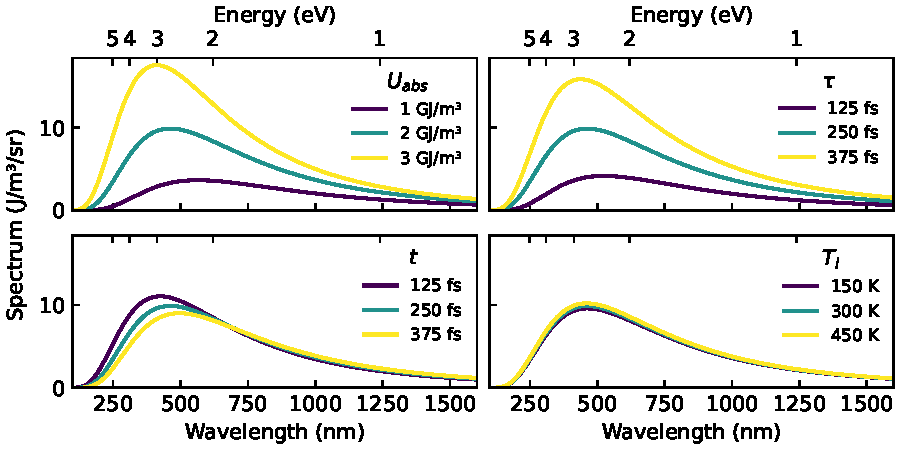
\includegraphics{../analysis/figures/sensitivity.pdf}
    \caption{}
    \label{fig:sensitivity}
\end{figure}
This model can be used to study how sensitive the spectrum to changes in the parameters. For this the spectrum is shown as before and with each parameter doubled and halved in \autoref{fig:sensitivity}.
The spectrum changes considerably with changes in the absorbed energy density $U_\text{abs}$ and the electron-phonon coupling time $\tau$. Changes in the excitation pulse time $\tau$ and the lattice temperature $T_l$ don't change the spectrum significantly.

\begin{figure}
    \centering
    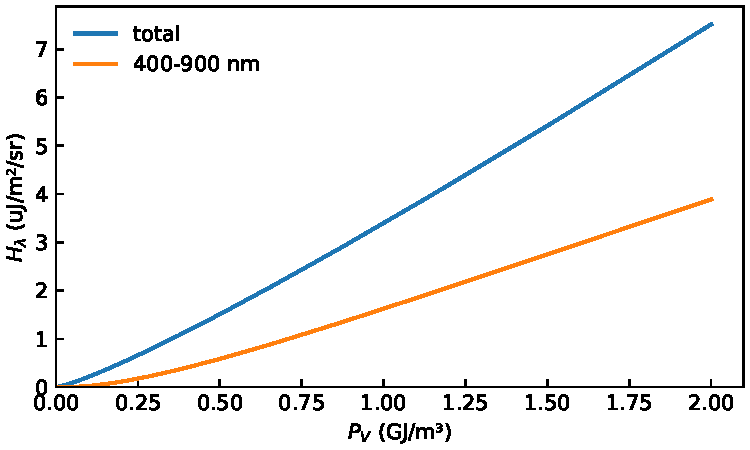
\includegraphics{../analysis/figures/powerscaling.pdf}
    \caption{}
    \label{fig:powerscaling}
\end{figure}
The dependence of the integrated spectrum $H$ on the absorbed power density is shown in more detail in \autoref{fig:powerscaling}.
When considering the total emitted power, it scales with absorbed energy. The flattening for low energies is due to the thermal radiation of the low lattice temperature $T_l$ becoming relevant.
We also show the emission detectable by a common detector.

\clearpage
\section{Experimental Setup}
\begin{figure}[h]
    \centering
    \begin{subfigure}{3.5in}
        \centering
        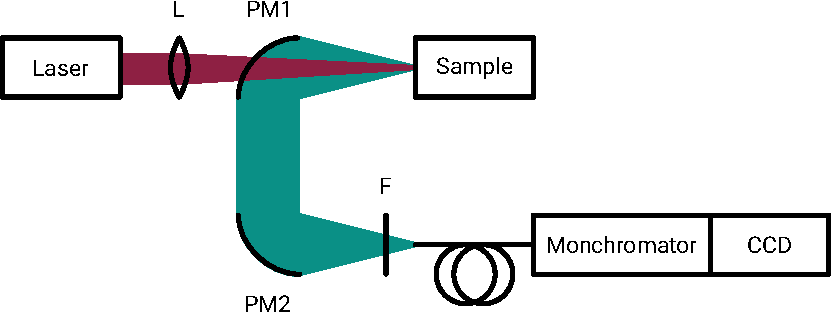
\includegraphics{figures/setup.pdf}
        \caption{Schematic}
    \end{subfigure}\hfill
    \begin{subfigure}{2in}
        \centering
        \includegraphics{figures/photo_setup.pdf}
        \caption{Photograph}
    \end{subfigure}
    \caption{Experimental setup used to measure thermal emission from ultrafast-excited hot electrons. The schematic shows the optical path and key components; the photograph shows the arrangement inside the chamber.}
    \label{fig:setup}
\end{figure}

The experimental setup, originally developed by Leon Roob~\cite{roobThermalRadiationUltrafast2025}, is shown in \autoref{fig:setup}. It is designed to measure broadband thermal emission from hot electrons in graphite using reflective collection optics and a fibre-coupled spectrometer.

The excitation source is a PHAROS PH1-20 (Light Conversion) at a centre wavelength of \SI{1030}{\nano\metre}, with pulse duration \SI{250}{\femto\second} (FWHM) and repetition rate \SI{40}{\kilo\hertz}. The pulse energy is \SI{7.5}{\micro\joule} (average power \SI{300}{\milli\watt}). The beam is stabilised in four axes and expanded to a diameter of $D=\SI{5}{\milli\metre}$ before entering the chamber.

Inside the chamber, a plano-convex lens with focal length \(f=\SI{200}{\milli\metre}\) focuses the beam onto the sample. Using the standard diffraction estimate \(d \approx 4\lambda f / \pi D\), the spot diameter is \(\SI{50}{\micro\metre}\).

The target is a graphite sample mounted on a three-axis translation stage. Thermal emission from the irradiated spot is collected by two off-axis parabolic mirrors (UV-enhanced aluminium). The first mirror (PM1, \(f=\SI{50}{\milli\metre}\)) collimates the emission; the second (PM2, \(f=\SI{101}{\milli\metre}\)) focuses it onto a band-pass filter and into a multimode fibre with a \SI{200}{\micro\metre} core (Ocean Optics QP200-2-SR-BX). The magnification is \(M = f_{\mathrm{PM2}}/f_{\mathrm{PM1}} \approx 2\), yielding an image spot of \(\sim\SI{100}{\micro\metre}\) at the fibre entrance, comfortably within the core.

The fibre feeds an Acton SpectraPro 300i monochromator equipped with a 150\,lines\,mm\(^{-1}\) grating blazed at \SI{500}{\nano\metre}. The dispersed spectrum is detected by an Andor iXon\textsuperscript{EM}+ 897 EMCCD operated in vertical binning mode, effectively serving as a 1D line detector.
Wavelength calibration (performed once following the manufacturer’s procedure~\cite{roobThermalRadiationUltrafast2025}) was stable throughout the measurements.

For alignment and maximal throughput, the lens, sample, and fibre ferrule are mounted on independent precision translation stages, while PM1 and PM2 are fixed on the common optical axis. 

\subsection{Noise and detector considerations}
Detecting the weak thermal radiation from hot electrons requires careful optimisation of the signal-to-noise ratio (SNR). In this setup the dominant noise sources originate from the detector; laser power fluctuations and mechanical variations are treated as negligible. The EMCCD mechanisms are well documented by Andor~\cite{dr.jowaltersSensitivityNoiseCCD2023,andorEstablishingSensitivityScientifica} and standards \cite{europeanmachinevisionassociationStandardCharacterizationImage2010}.

\textbf{Readout noise.}
This is the fundamental noise from charge transfer and A/D conversion. For the present camera, the fit in \autoref{fig:dark_noise} yields a constant read noise of
\(\sigma_{\text{read}}=\SI{0.81(12)}{DN}\), consistent with the manufacturer’s specification~\cite{andorIXonEM897Manual}.
Because read noise is applied per read out bin, hardware binning (1D line-detector mode) reduces its impact by summing signal prior to the single read.

\textbf{Dark current noise.}
Thermally generated charge scales with temperature and time,
\(N_\text{dark}\propto \exp(-E/kT)\,t_\text{exp}\).
\autoref{fig:dark_noise} shows the measured dependence; fitting gives an effective activation energy \(E=\SI{0.597(4)}{eV}\).
With the sensor cooled to \SI{-80}{\degreeCelsius}, the dark contribution is negligible at the exposure times used.

\begin{figure}[h]
    \centering
    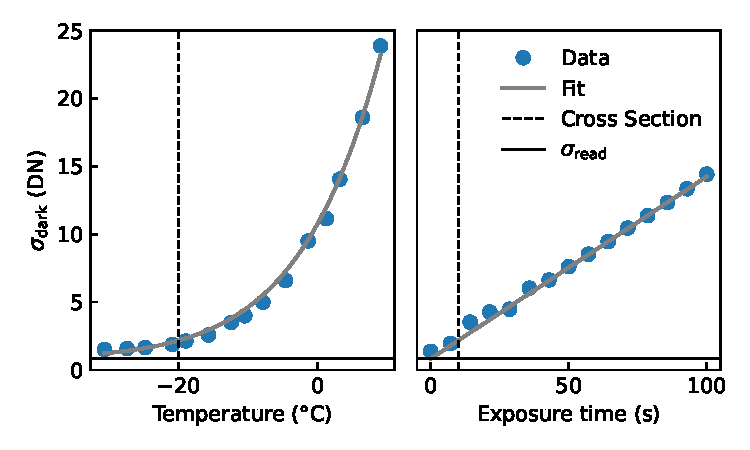
\includegraphics{../analysis/figures/dark_noise.pdf}
    \caption{Dark noise vs.\ sensor temperature and exposure time. Fit yields \(E=\SI{0.597(4)}{eV}\) and \(\sigma_{\text{read}}=\SI{0.81(12)}{e^{-}}\).}
    \label{fig:dark_noise}
\end{figure}

\textbf{Clock-induced charge (CIC).}
CIC is created during high-speed clocking.
Its apparent contribution grows with electron multiplication gain, so \emph{EM gain is disabled} in this work (signal levels are well above the read-noise floor), which keeps CIC negligible~\cite{andorEstablishingSensitivityScientifica}.

\textbf{Shot noise and photon-transfer method.}
Under these optimised conditions the dominant term is shot noise.
Incident photons create photoelectrons with quantum efficiency \(\eta\), so \(N_e=\eta\,N_{\text{photons}}\) and, for Poisson statistics, \(\operatorname{var}(N_e)=N_e\)~\cite{europeanmachinevisionassociationStandardCharacterizationImage2010}.
Let \(G\) denote the system conversion gain (DN per electron). The measured signal in data numbers (DN) is \(S = G\,N_e\), and the measured variance becomes \(\sigma^2_{\text{meas}} \;=\; \sigma_{\text{read}}^2 \;+\; G\,S\).
Thus a plot of variance vs.\ mean (photon-transfer curve) is linear in the shot-noise regime with slope \(G\).
\autoref{fig:shotnoise} shows this behaviour; from the slope \(G \approx 10~\text{DN}/e^{-}\) can be measured.
Note that this procedure does \emph{not} determine \(\eta\); it only gives the DN-to-electron conversion.

\begin{figure}[h]
    \centering
    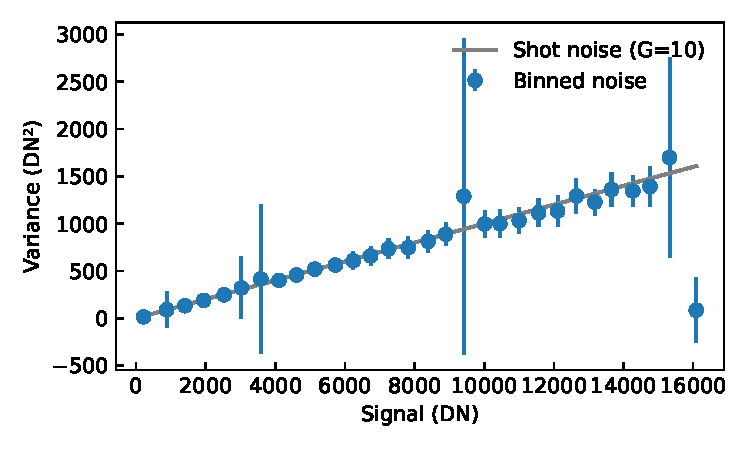
\includegraphics{../analysis/figures/shot noise.pdf}
    \caption{Measured noise vs.\ signal (photon-transfer curve) demonstrating shot-noise-limited operation; the linear slope yields the conversion gain \(G\).}
    \label{fig:shotnoise}
\end{figure}

\textbf{Practical settings for reproducibility.}
(1) Keep the camera at \(\leq\)\SI{-80}{\degreeCelsius}; (2) use vertical binning to treat the EMCCD as a 1D detector; (3) disable EM gain to avoid CIC and excess-noise-factor penalties; (4) fix slit width and exposure during noise characterisation; (5) verify the shot-noise regime by measuring \(\sigma^2\) vs.\ \(S\) and confirming linearity and slope \(G\)

\subsection{Focusing and Alignment}
The aim is to image the excited spot on the sample onto the spectrometer fibre with maximal throughput. Parabolic mirrors (PM1/PM2) remain fixed once set; all focusing is done with the lamp, fibre/spectrometer port, and sample stages.

\begin{enumerate}
  \item \textbf{Initial setup with a fiber coupled lamp.}  
  Remove the sample and place a fiber-coupled lamp at the sample position. This will help align and focus the optics using visible light.

  \item \textbf{Align the beam.}  
  Adjust the lamp position and the parabolic mirrors so that the beam appears circular and sharply focused at the spectrometer fiber port. This ensures the optics are approximately aligned.

  \item \textbf{Connect and optimize with spectrometer.}  
  Connect the spectrometer to the spectrometer port and move the holder to maximize the signal roughly. Use the micrometer screws on the sample stage for fine adjustments.

  \item \textbf{Swap back in the sample.}  
  Replace the lamp with the sample at the same position. Connect the lamp output to the spectrometer port to illuminate the sample.

  \item \textbf{Fine-focus the sample.}  
  Adjust the sample position to minimize the size of the visible spot on the sample.

  \item \textbf{Focus the infrared laser.}  
  Turn on the infrared laser and use an IR detection card to locate and focus the beam onto the sample. The white light and the IR be collinear.

  \item \textbf{Optimize laser alignment.}  
  Replace the lamp with the spectrometer and monitor the reflected laser signal on the spectrometer. Fine-tune the laser focus to maximize this signal.
\end{enumerate}

\subsection{Data processing}
All raw spectra were first corrected by subtracting a dark frame recorded with identical acquisition settings, removing the fixed electronic bias and dark current.  
Residual peaks at the fundamental and harmonic wavelengths of the pump laser, normally suppressed by laser line filters, were present due to the absence of suitable optical filtering.  
These peaks were identified and removed digitally, leaving gaps in the plotted spectra where the affected bins were excluded.  

The corrected signal \(S(\lambda)\) in DN was converted to spectral power density \(P_{\text{meas}}(\lambda)\) via
\begin{equation}
  P_{\text{meas}}(\lambda)
  = \frac{S(\lambda)}{G\,t_{\text{exp}}\,\Delta\lambda}\,\frac{hc}{\lambda},
\end{equation}
with \(G\) the DN/\(e^-\) conversion gain, \(t_{\text{exp}}\) the exposure time, and \(\Delta\lambda\) the spectral bin width.  

\clearpage
\section{Measurement}
\begin{figure}[h]
    \centering
    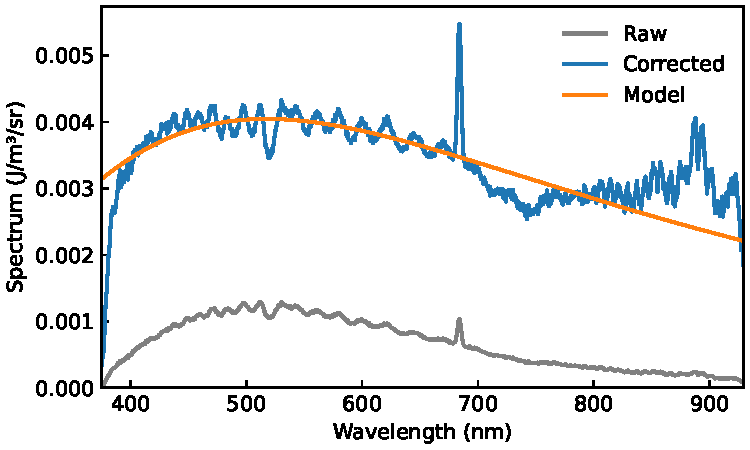
\includegraphics{../analysis/figures/combined.fit.pdf}
    \caption{}
    \label{fig:fit}
\end{figure}
Before comparing the model with the measurement, the raw measurement (shown in \autoref{fig:fit}) has to be corrected with the instruments calibration curve.
This contains the manufacturer supplied efficiency of the camera \cite{andorIXonEM897Manual} and the efficiency curve of the monochromator.
This is modelled using \autocite{barkerRippleCorrectionHighdispersion1984} and the unknown model parameter $k=1.18$ fitted by minimizing the error between the corrected spectrum and the model.
The model and the fitted corrected spectrum is also shown in \autoref{fig:fit}.
The model was scaled by $0.2$ and the absorbed energy density $U_\text{abs} = \SI{1.93e9}{J/m^3}$ fitted to the measurement.

It is not surprising that the model has a higher scale than the measurement, as some losses (e.g. fiber coupling) are not accounted for.
The incident energy density $U_\text{inc} = P_\text{avg} \; / \; f_\text{rep} \pi r_\text{spot}^2 d = \SI{4.8e9}{J/m^3}$ with the average Power $P_\text{avg}=\SI{300}{mW}$, the repetition rate $f_\text{rep}=\SI{40}{kHz}$, the spot size $r_\text{spot}=\SI{50}{\micro m}$ and the absorption depth $d=\SI{200}{nm}$ \cite{smauszDeterminationUVVisible2017} is more due to some light being reflected and scattered. It correspondence with a incident fluence of \SI{950}{J/m^2}. 

The light around \SI{900}{nm} and the peak at peak at \SI{688}{nm} in the corrected spectrum may be due to the laser light not being filtered before reaching the sample.

\section{Discussion and Conclusion}

\clearpage
\printbibliography

\end{document}